\documentclass[10pt,twoside,slovak,a4paper]{article}

\usepackage[slovak]{babel}
\usepackage[IL2]{fontenc} % lepšia sadzba písmena Ľ než v T1
\usepackage[utf8]{inputenc}
\usepackage{graphicx}
\usepackage{url} % príkaz \url na formátovanie URL
\usepackage{hyperref} % odkazy v texte budú aktívne (pri niektorých triedach dokumentov spôsobuje posun textu)
\usepackage{cite}
\usepackage{listings}
%\usepackage{times}

\pagestyle{headings}

\title{Praktická aplikácia regulárnych výrazov. Problémy a ťažkosti pri ich písaní a používaní.\thanks{Semestrálny projekt v predmete Metódy inžinierskej práce, ak. rok 2023/24, vedenie: PaedDr. Pavol Baťalík}} % meno a priezvisko vyučujúceho na cvičeniach

\author{Denis Danilov\\[2pt]
	{\small Slovenská technická univerzita v Bratislave}\\
	{\small Fakulta informatiky a informačných technológií}\\
	{\small \texttt{xdanilovd@stuba.sk}}}
\date{\small \today} % upravte

\begin{document}
\maketitle
\begin{abstract}
Regulárne výrazy, často známe ako regex, je formálny jazyk, ktorý sa používa na priraďovanie textových vzorov. Používanie regexov pomáha rýchlo a presne nájsť a extrahovať kľúčové informácie z veľkých objemov textu. Môžu Vám doslova pomôcť nájsť ihlu v kope sena, čo organizáciám umožňuje presmerovať svoje ľudské zdroje do iných oblastí. Regexy sú obzvlášť užitočné na definovanie filtrov, pretože obsahujú postupnosť znakov, ktoré definujú vzor textu, ktorý sa má zhodovať.
Cieľom tejto práce je preskúmať, ako sa regulárne výrazy často používajú v praxi, identifikovať problémy a ťažkosti, s ktorými sa programátori stretávajú pri písaní a používaní regulárnych výrazov.
Metódami na dosiahnutie cieľa bude analýza prieskumu medzi vývojármi a údajov o používaní regulárnych výrazov v otvorených projektoch na GitHub.
Tento článok jasne ukáže výhody používania regulárnych výrazov, ako aj osvedčené postupy pri ich písaní.
\end{abstract}

\section{Úvod}
Regulárne výrazy, tiež známe ako Regexy, sú nástrojom na spracovanie textu, ktorý je integrovaný do všetkých súčasných programovacích jazykov a bežne používaných utilít, ako sú textové editory. Regulárne výrazy sa používajú pri úlohách vyhľadávania a nahrádzania reťazcov, ako je vyhľadávanie slov, úprava textu a analýza súborov. \cite{Chapman2017}
Odhady naznačujú, že viac ako tretina projektov JavaScript a Python obsahuje aspoň jeden regulárny výraz. \cite{Michael2019} \\
\\
Regulárne výrazy sú široko používané v rôznych oblastiach výpočtovej techniky. Tu je niekoľko bežných prípadov použitia:
\begin{enumerate}
	\item \textbf{Analýza protokolov:} Regulárne výrazy možno použiť na extrahovanie špecifických častí informácií zo systémových alebo aplikačných protokolov.
	\item \textbf{Overenie údajov:} Môžu sa použiť na overenie formátu vstupných údajov, ako sú e-mailové adresy, telefónne čísla a ID používateľov.
	\item \textbf{Hľadať a nahradiť:} Regulárne výrazy možno použiť na nájdenie a nahradenie konkrétnych vzorov v texte alebo kódovej základni.
	\item \textbf{Premenovanie súborov:} Môžu sa použiť na dávkové premenovanie súborov na základe určitých vzorov.
	\item \textbf{Analýza vstupu používateľa:} Regulárne výrazy možno použiť na analýzu vstupu používateľa alebo príkazových riadkov.
	\item \textbf{Čítanie konfiguračných súborov:} Môžu sa použiť na čítanie a analýzu konfiguračných súborov.
\end{enumerate}
Pochopenie a písanie regulárnych výrazov si vyžaduje znalosti aj zručnosti. \cite{Chapman2016}
Jediná chyba v znaku môže spôsobiť drasticky odlišné správanie regulárneho výrazu pri porovnávaní. \cite{Wang2019}
Viac ako 80 \% regulárnych výrazov napísaných v projektoch GitHub však nie je otestovaných \cite{Wang2018}, čo naznačuje, že vývojári buď regulárne výrazy netestujú, alebo namiesto testovacích prípadov používajú externé nástroje. \cite{Wang2019} \\
\\
Pre regulárne výrazy \cite{5477051} existujú nástroje na generovanie testov regulárnych výrazov. Tieto nástroje vymenúvajú členy jazyka regulárnych výrazov, ale nevypočítavajú nezhodujúce sa reťazce. Nedávne výskumné úsilie skúmalo prístup založený na chybách pri generovaní testov regulárnych výrazov prostredníctvom testovania mutácií \cite{7899040}; do regulárnych výrazov sa vnášajú chyby a generujú sa reťazce, ktoré sú svedkami chyby, čím sa poskytujú príklady nezhodného správania pôvodného regulárneho výrazu. Hoci je testovanie mutáciou zrelou oblasťou výskumu, na mutáciu regulárnych výrazov sa zamerali nedávno \cite{7899040} \cite{7374717}. Tieto snahy však definovali operátory mutácie ad hoc spôsobom, bez toho, aby zohľadnili, ako sa regulárne výrazy v praxi skutočne vyvíjajú. Preto injektované chyby nemusia byť reprezentatívne pre skutočné úpravy.\cite{Wang2019}\\
\\
Tento článok je určený na to, aby vám pomohol pochopiť a efektívne používať regulárne výrazy.  Začneme základnými pojmami a postupne prejdeme k pokročilejším príkladom.

\section{Výskumné úlohy}
V tejto práci používame termín reprezentácia regexu na označenie syntaktického vyjadrenia regulárneho výrazu. Funkcia je štrukturálna zložka regulárneho výrazu (napr. Kleenova hviezdička: * alebo vlastná trieda znakov: \cite{Chapman2017}). Trieda ekvivalencie je skupina behaviorálne ekvivalentných regulárnych výrazov. Pri skúmaní porozumenia regexov odpovedáme na nasledujúce výskumné otázky: \cite{Chapman2017}\\\\
\begin{figure}[h]
	\centering
	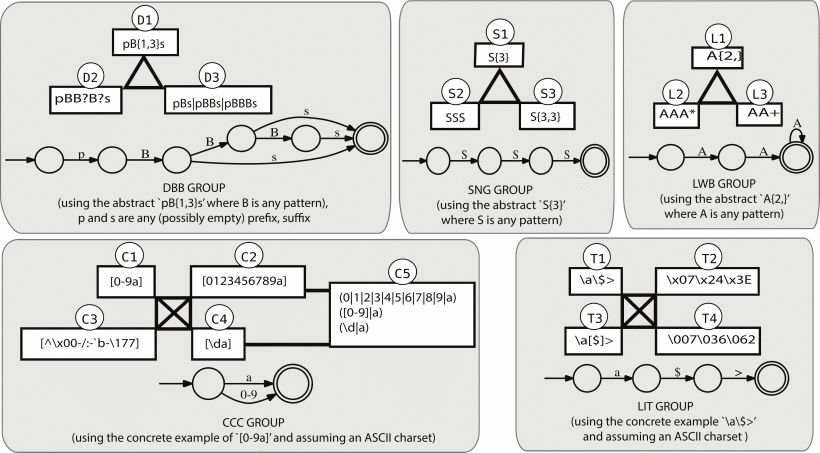
\includegraphics[width=0.5\textwidth]{obrazok1.png}
	\caption{Typy tried ekvivalencie na základe vlastností jazyka. DBB = dvojnásobne ohraničená, SNG = jednoduchá ohraničená, LWB = nižšia ohraničená, CCC = vlastná trieda znakov a LIT = literálna. Na ilustráciu používame konkrétne regexy spolu s ich deterministickým konečným automatom (dfa) v reprezentáciách. A v skupine LWB (alebo B v skupine DBB, S v skupine SNG a podobne) však abstraktne reprezentujú akýkoľvek vzor, s ktorým by sa dalo pracovať modifikátorom opakovania (napr. literálne znaky, triedy znakov alebo skupiny). To isté platí pre literály používané vo všetkých reprezentáciách. \cite{Chapman2017}}
	\label{fig:obrazok1}
  \end{figure}
\textbf{} \\\\

\textbf{Ktoré reprezentácie regexov sú najzrozumiteľnejšie?} \\\\
Aby sme odpovedali na prvú otázku, uskutočnili sme štúdiu, v ktorej sme programátorom predložili regex a položili im otázky o jeho správaní pri porovnávaní. Porovnaním presnosti regexov, ktoré zodpovedajú rovnakému jazyku, ale sú vyjadrené pomocou rôznych reprezentácií (napr. tri[a-f] 3 a tri (a \textbar \ b \textbar \ c \textbar \ d \textbar \ e \textbar \ f)3), môžeme merať zrozumiteľnosť a identifikovať zápach kódu. \cite{Chapman2017} \\
Skúmame aj faktory, ktoré môžu ovplyvniť porozumenie, konkrétne dĺžku reťazca regexu, veľkosť regexu DFA (Deterministický konečný automat) a reprezentáciu triedy ekvivalencie. Táto analýza si vyžaduje identifikáciu tried ekvivalencie pre regexy. Kontrolou súboru údajov o regexoch v jazyku Python, ktorý obsahuje takmer 14 000 regexov \cite{Chapman2016}, sme vytvorili počiatočný súbor piatich typov tried ekvivalencie, ktoré sme skúmali.\cite{Chapman2017}\\\\
\textbf{Ktoré reprezentácie regexov majú najväčšiu podporu komunity na základe frekvencie?} \\\\
Na zodpovedanie druhej otázky skúmame verejne dostupný súbor údajov o regexoch \cite{Chapman2016} a používame prítomnosť a neprítomnosť jazykových znakov ako zástupný ukazovateľ podpory komunity, pričom sa predpokladá, že častejšie používané znaky sú zrozumiteľnejšie.\cite{Chapman2017}\\\\

\section{Základy písania regulárnych výrazov}
\subsection{Ako vyzerá regulárny výraz?}
V najjednoduchšej podobe môže regulárny výraz vyzerať takto:
\begin{lstlisting}[frame=single, basicstyle=\ttfamily\small, label=code:example]
	/Test/
	\end{lstlisting}

V príklade "Test" vygeneroval test písmena podobný vzor vyhľadávania ako pri jednoduchom vyhľadávaní.
Tieto regulárne výrazy však nie sú vždy také jednoduché. Tu je regulárny výraz, ktorý zodpovedá 3 číslam, za ktorými nasleduje znak "-", potom 3 čísla, za ktorými nasleduje ďalší znak "-" a nakoniec končí 4 číslami.
\begin{lstlisting}[frame=single, basicstyle=\ttfamily\small, label=code:example]
	^(?:\d{3}-){2}\d{4}$
	\end{lstlisting}

Väčšinu regulárnych výrazov možno v skutočnosti zapísať viacerými spôsobmi, rovnako ako iné formy programovania. Napríklad vyššie uvedený sa dá prepísať do dlhšej, ale o niečo čitateľnejšej verzie:
\begin{lstlisting}[frame=single, basicstyle=\ttfamily\small, label=code:example]
	^[0-9]{3}-[0-9]{3}-[0-9]{4}$
	\end{lstlisting}

Väčšina jazykov poskytuje zabudovanú metódu na vyhľadávanie a nahrádzanie reťazcov pomocou regulárnych výrazov. Každý jazyk však môže mať iný súbor syntaxe v závislosti od toho, čo daný jazyk predpisuje.\\
V tomto článku sa zameriame na variant regulárneho výrazu ECMAScript, ktorý sa používa v jazyku JavaScript a má veľa spoločného s implementáciami regulárnych výrazov v iných jazykoch.

\subsection{Ako čítať (a zapisovať) regulárne výrazy}
\subsubsection{Kvantory}
Kvantifikátory regulárnych výrazov kontrolujú, koľkokrát sa má znak vyhľadať.\\
Tu je zoznam všetkých kvantifikátorov:\\
\begin{itemize}
	\item a \textbar \ b - Zodpovedajúce ''a" \ alebo ''b".
	\item ? - Nula alebo jednotka
	\item + - jedna alebo viac
	\item * ? Nula alebo viac?
	\item {N} - Presne N-krát (kde N je číslo)
	\item {N,} - N alebo viac krát (kde N je číslo)
	\item {N,M} - N až M krát (kde N a M sú čísla a N \textless \ M)
	\item *? - Nula alebo viac, ale zastavenie po prvej zhode
	\end{itemize}

Napríklad nasledujúci regulárny výraz:
\begin{lstlisting}[frame=single, basicstyle=\ttfamily\small, label=code:example]
	Ahoj \textbar Dobre
	\end{lstlisting}
Zodpovedá reťazcom ''Ahoj" \  a ''Dobre".\\\\
Medzitým:
\begin{lstlisting}[frame=single, basicstyle=\ttfamily\small, label=code:example]
	Ahoj?
	\end{lstlisting}
Bude sledovať ''j" \ od nuly do jednej, takže bude zodpovedať ''Aho" \ a ''Ahoj".\\\\
Alternatívne:
\begin{lstlisting}[frame=single, basicstyle=\ttfamily\small, label=code:example]
	Ahoj{1,3}
	\end{lstlisting}
Bude zodpovedať ''Ahoj", ''Ahojj", ''Ahojjj", ale nie ''Ahojjjj", pretože hľadá písmeno ''j" \ od 1 do 3 krát.
\subsubsection{Chamtivé porovnávanie}
Jedným z kvantifikátorov regexu, ktorého sme sa dotkli v predchádzajúcom zozname, bol symbol. Tento symbol zodpovedá jednému alebo viacerým znakom. To znamená, že:+
\begin{lstlisting}[frame=single, basicstyle=\ttfamily\small, label=code:example]
	Ahoj+
	\end{lstlisting}
	Zodpovedá všetkým slovám od ''Ahoj" \ po ''Ahojjjjjjjjjjjj". Je to preto, že všetky kvantifikátory sú štandardne považované za ''chamtivé".
	Ak ho však zmeníte na "lenivý" pomocou symbolu otáznika () na nasledujúci, správanie sa zmení?
\begin{lstlisting}[frame=single, basicstyle=\ttfamily\small, label=code:example]
	Ahoj+?
	\end{lstlisting}
	Teraz sa porovnávač pokúsi nájsť zhodu čo najmenej krát. Keďže ikona znamená ''jeden alebo viac", bude sa zhodovať len s jedným ''j". To znamená, že ak zadáme reťazec''Ahojjjjjjjjjjjj", porovná sa iba ''Ahoj".i+\\
    Hoci to samo o sebe nie je obzvlášť užitočné, v kombinácii so širšími zhodami, ako je symbol, sa to stáva mimoriadne dôležitým, ako si povieme v nasledujúcej časti. Symbol sa v regexe používa na nájdenie''akéhokoľvek znaku".\\
	Ak teraz použijete:
\begin{lstlisting}[frame=single, basicstyle=\ttfamily\small, label=code:example]
	A.*oj
	\end{lstlisting}
	Môžete porovnať všetko od ''Achoj" \ po ''Ahoj" \ aj po ''Ahojchojhoj".

\subsubsection{Zbierky vzorov}
Zbierky vzorov umožňujú vyhľadať kolekciu znakov, ktoré sa majú porovnať. Napríklad pomocou nasledujúceho regexu:
\begin{lstlisting}[frame=single, basicstyle=\ttfamily\small, label=code:example]
	Moja oblubena hlaska je [aeiou]
	\end{lstlisting}
	Môžete porovnať nasledujúce reťazce:
	\begin{lstlisting}[frame=single, basicstyle=\ttfamily\small, label=code:example]
		Moja oblubena hlaska je a
		Moja oblubena hlaska je e
		Moja oblubena hlaska je i
		Moja oblubena hlaska je o
		Moja oblubena hlaska je u
		\end{lstlisting}
Ale nič iné.\\
Tu je zoznam najbežnejších zbierok vzorov:
\begin{itemize}
	\item \ [A-Z] - Zodpovedá akémukoľvek veľkým písmenám od ''A" \ po ''Z".
	\item \ [a-z] - Zodpovedá akémukoľvek malým písmenám od ''a" \ po ''z".
	\item \ [0-9] - Zodpovedá akýmkoľvek číslam.
	\item \ [asdf] - Zodpovedá akémukoľvek znaku, ktorý je buď ''a", ''s", ''d" \ alebo ''f".
	\item \ [\textasciicircum asdf] - Zodpovedá akémukoľvek znaku, ktorý nie je ''a", ''s", ''d" \ alebo ''f".
  	\end{itemize}
\subsubsection{Všeobecné tokeny}
Nie každá postava je tak ľahko identifikovateľná. Kým kľúče ako "a" až "z" majú zmysel priradiť pomocou regexu, ako je to so znakom nového riadku?
\begin{itemize}
	\item . - Akýkoľvek znak
	\item \textbackslash n - Znak nového riadka
	\item \textbackslash t - Znak tabulácie
	\item \textbackslash s - Akýkoľvek medzerníkový znak znak (vrátane medzier a iných)
	\item \textbackslash S - Akýkoľvek znak, ktorý nie je medzerníkový
	\item \textbackslash w - Akýkoľvek znak slova (veľké a malé písmená latinskej abecedy, číslice 0-9 a \textunderscore )
	\item \textbackslash W - Akýkoľvek znak, ktorý nie je znakom slova
	\item \textbackslash b - Hraničný znak slova: hraničné znaky medzi w a \textbackslash W, ale zhoduje sa so znakmi medzi znakmi \textbackslash w \textbackslash W
	\item \textbackslash B - Hraničný znak slova: opak znaku \textbackslash b
	\item \textasciicircum \ - Začiatok riadka
	\item \$ - Koniec riadka
	\item \textbackslash \textbackslash \ - Doslovný znak ''\textbackslash"
 	\end{itemize}
	 Ak by ste teda chceli odstrániť každý znak, ktorý začína nové slovo, mohli by ste použiť niečo ako nasledujúci regex:\\
\begin{lstlisting}[frame=single, basicstyle=\ttfamily\small, label=code:example]
	\s.
	\end{lstlisting}
	A výsledky nahraďte prázdnym reťazcom. Pri tomto postupe je nasledovné:
\begin{lstlisting}[frame=single, basicstyle=\ttfamily\small, label=code:example]
	Ahoj ako sa mas
	\end{lstlisting}
	Stáva sa:
\begin{lstlisting}[frame=single, basicstyle=\ttfamily\small, label=code:example]
	Ahojkoaas
	\end{lstlisting}

Kombináciou uvedených metód môžete vyriešiť väčšinu základných úloh, s ktorými sa vývojár stretáva.

\section{Štúdia o zrozumiteľnosti}
Táto štúdia predstavuje programátorom regexy a kladie otázky na porozumenie. Porovnaním zrozumiteľnosti sémanticky ekvivalentných regexov, ktoré zodpovedajú rovnakému jazyku, ale majú rôzne syntaktické reprezentácie, sa snažíme identifikovať zápachy kódu. Táto štúdia bola realizovaná na portáli Amazon Mechanical Turk so 180 účastníkmi. Celkovo sa hodnotilo 60 regexov, čím sa vytvorilo 42 párov porovnávania regexov. Každý regexový vzor hodnotilo 30 účastníkov. \cite{Chapman2017}
\begin{figure}[h]
	\centering
	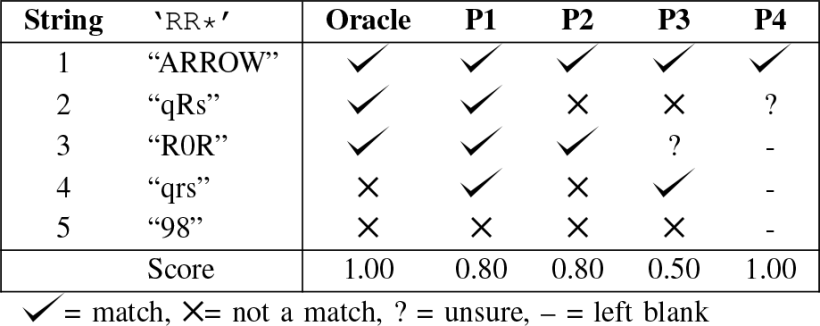
\includegraphics[width=0.5\textwidth]{Table I.png}
	\caption{Príklad metrického porovnávania \cite{Chapman2017}}
	\label{fig:table1}
  \end{figure}
\subsection{Metriky}
Zrozumiteľnosť regexov meriame pomocou dvoch komplementárnych metrík, porovnávania a skladania. Tieto metriky sa označujú ako metriky zrozumiteľnosti. Pre hlbší pohľad na údaje s cieľom lepšie pochopiť faktory, ktoré ovplyvňujú zrozumiteľnosť, vypočítame aj dĺžku regexu a veľkosť DFA pre každý regex.\cite{Chapman2017}
\subsubsection{Zodpovedanie}
Pri danom vzore a množine reťazcov účastník kontrolou určí, ktoré reťazce sa budú zhodovať so vzorom. Pre každý reťazec existujú štyri možné odpovede: zodpovedá, nezodpovedá, nie je istý alebo je prázdny. Príklad z našej štúdie je uvedený \hyperref[fig:obrazok2]{na obrázku 2}.\cite{Chapman2017}\\\\
Percentuálny podiel správnych odpovedí, bez zohľadnenia prázdnych miest a neistých odpovedí, predstavuje skóre zhody. Uvažujme napríklad regexový vzor "RR*, päť reťazcov uvedených v tabuľke I a odpovede štyroch účastníkov v stĺpcoch Pl,P2,P3 a P4. Oracle uvádza, že prvé tri reťazce sa zhodujú a posledné dva nie; Pl odpovedá správne na prvé tri reťazce a piaty, ale nesprávne na štvrtý, takže skóre zhody je 4/5=0,80. P2 si nesprávne myslí, že druhý reťazec sa nezhoduje, takže skóre je tiež 4/5=0,80. P3 označí tretí reťazec ako "neistý", takže celkový počet pokusov o zhodu je 4. P3 sa nesprávne vyjadrí o druhom a štvrtom reťazci, takže dosiahne skóre 2/4=0,50. V prípade P4 máme k dispozícii údaje len pre prvý a druhý reťazec, pretože ostatné tri sú prázdne. P4 označí druhý reťazec ako "neistý", takže sa pokúsil zodpovedať len jednu otázku; skóre za zhodu je 1/1=1,00.\cite{Chapman2017}\\\\
Do metriky boli zahrnuté prázdne miesta, pretože v štúdii sa občas vyskytli nevyplnené otázky. Neisté odpovede boli uvedené ako možnosť, aby nedošlo k skresleniu výsledkov slepým odhadom. Tieto situácie sa nevyskytovali veľmi často. Z 1 800 otázok (180 účastníkov * 10 otázok) bolo iba 1,8 \% (32) ovplyvnených prázdnou alebo neistou odpoveďou (nikdy nie viac ako štyri z 30 odpovedí na vzor). \cite{Chapman2017}
\begin{figure}[h]
	\centering
	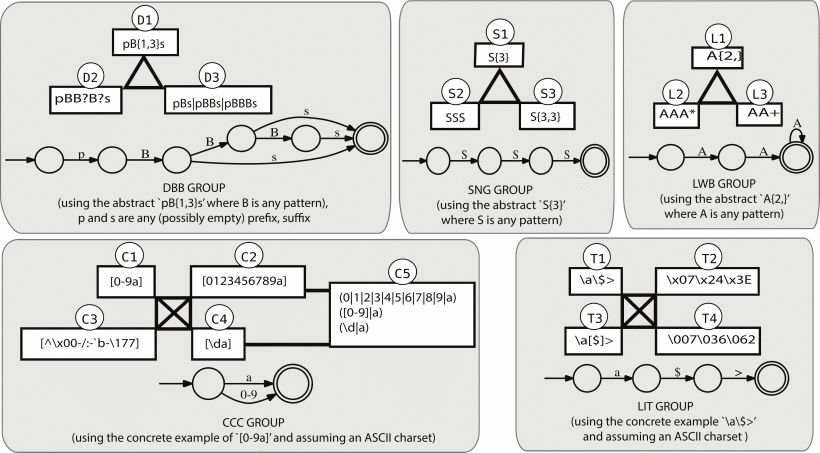
\includegraphics[width=0.5\textwidth]{obrazok1.png}
	\caption{Otázky z jedného vzoru na jeden zásah \cite{Chapman2017}}
	\label{fig:obrazok2}
  \end{figure}
\subsubsection{Zloženie}
Ak je daný vzor, účastník vytvorí reťazec, o ktorom si myslí, že sa mu zhoduje (otázka 7.F \hyperref[fig:obrazok2]{na obrázku 2}). Ak je účastník presný, skóre zloženia je 1, inak 0. Napríklad vzhľadom na vzor (q4fab \textbar ab) z našej štúdie sa reťazec "xyzq4fab" zhoduje a získa skóre 1, ale reťazec "acb" sa nezhoduje a získa skóre 0.\cite{Chapman2017}\\\\
Na určenie zhody medzi reťazcom a vzorom sa vzor skompiluje pomocou modulu re.compile v jazyku Python. Pomocou skompilovaného vzoru sa vytvorí inštancia re.RegexObject m. m.search() vráti inštanciu re.MatchObject m2 s reťazcom zadaným ako vstup do tejto funkcie. Ak m2 nie je None, potom je tento reťazec zhodný a má hodnotu 1; v opačnom prípade má hodnotu 0.\cite{Chapman2017}
\subsubsection{Dĺžka regexu}
Pri danom vzore sa dĺžka regexu vypočíta podľa dĺžky jeho literálneho reťazca. Napríklad regexy \textbackslash 072 a ab*c majú dĺžku štyri.\cite{Chapman2017}
\subsubsection{Veľkosť DFA}
Aby sme vypočítali veľkosť minimálneho DFA, na každom regexe spustíme brics  aj Rex \cite{5477051} a ručne skontrolujeme ich výsledky, aby sme zaručili ich správnosť.\cite{Chapman2017}
\subsection{Dizajn}
Túto štúdiu sme realizovali na platforme Amazon Mechanical Turk (MTurk), na ktorej žiadatelia vytvárajú úlohy ľudskej inteligencie (HIT), ktoré majú pracovníci dokončiť.\cite{Chapman2017}
\subsubsection{Kvalifikácia pracovníka}
Kvalifikovaní pracovníci museli správne odpovedať na štyri z piatich základných otázok regexu. Tieto otázky boli s výberom odpovede a pracovník mal analyzovať tieto vzory: a+, (r \textbar \ z), \textbackslash \textbackslash \textbackslash \textbackslash \textbackslash \textbackslash \textbackslash \textbackslash d, q* a [p-s].\cite{Chapman2017}
\subsubsection{Úlohy}
Na základe vzorov v korpuse sme vytvorili 60 regexových vzorov, ktoré sme zoskupili do 26 skupín sémantickej ekvivalencie. V 18 skupinách boli dva regexy zamerané na rôzne hrany v triedach ekvivalencie. Ďalších osem skupín malo po tri regexy. Celkovo bolo vytvorených 42 dvojíc vzorov. Takto môžeme vyvodiť závery porovnaním reprezentácií, keďže vyhodnotené regexy boli sémanticky ekvivalentné.\cite{Chapman2017} \\\\
Na vytvorenie sémantických skupín sme vzali regex z korpusu, priradili sme ho k reprezentácii na \hyperref[fig:obrazok1]{obrázku 1}, skrátili sme ho tak, aby obsahoval len o málo viac než len funkciu, ktorá nás zaujíma, a potom sme vytvorili ďalšie regexy, ktoré sú sémanticky ekvivalentné, ale patria do iných uzlov triedy ekvivalencie. Napríklad sémantická skupina s regexmi ((q4f) {0, 1} ab, ((q4f) ?ab) a (q4fab \textbar ab) patrí do D1, D2 a D3. Skupina s regexmi ([0-9] +) \textbackslash . ([0-9] +) a (\textbackslash d+) \. (\textbackslash d+) je určená na vyhodnotenie hrany medzi C1 a C4. Poznamenávame, že ak by sme použili len regexy z korpusu, mali by sme v každom uzle regexy s rôznou sémantikou alebo s ďalšími jazykovými vlastnosťami, čo by sťažilo porovnávanie cieľových vlastností.\cite{Chapman2017}
\begin{figure}[h]
	\centering
	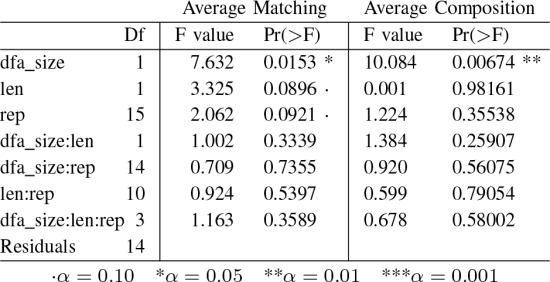
\includegraphics[width=0.5\textwidth]{table2.png}
	\caption{3-faktorová anova s priemernou presnosťou zhody alebo zloženia ako závislými premennými, pri zohľadnení reprezentácie (REP), veľkosti DFA (dfa \textunderscore size) a dĺžky regexu (len) ako nezávislých premenných \cite{Chapman2017}}
	\label{fig:table2}
  \end{figure} \\
Pre každú z 26 sémantických skupín sme vytvorili päť reťazcov pre štúdiu, kde sa aspoň jeden zhodoval a aspoň jeden nezhodoval. Tie sa použili na výpočet metriky zhody. Po zhromaždení všetkých vzorov a zhodných reťazcov sme vytvorili úlohy pre účastníkov MTurk nasledovne: náhodne vybrať vzor z 10 z 26 sémantických skupín. Náhodne vyberte poradie týchto 10 vzorov, ako aj poradie zodpovedajúcich reťazcov pre každý vzor. Po pridaní otázky, v ktorej sa účastník pýta na zloženie reťazca, ktorý zodpovedá každému vzoru, sa tak vytvorí jedna úloha na MTurku, ako je príklad na \hyperref[fig:obrazok2]{na obrázku 2}. Tento proces sa dokončil, kým sa každý zo 60 regexov neobjavil v 30 HIT, čo viedlo k celkovému počtu 180 jedinečných HIT.\cite{Chapman2017}
\subsubsection{Implementácia}
Pracovníci dostali 3,00 USD za úspešné absolvovanie jedného a len jedného HIT. Priemerný čas dokončenia prijatých HIT bol 682 sekúnd (11 min. 22 s). Celkovo bolo odmietnutých 54 HIT: 48 malo príliš veľa prázdnych odpovedí, štyri boli dvojnásobné podania od tých istých pracovníkov, jeden neodpovedal na otázky týkajúce sa zloženia a v jednom chýbali údaje z 3 otázok. Odmietnuté HIT-y boli vrátené na MTurk, aby ich vyplnili iní.\cite{Chapman2017}
\subsubsection{Účastníci}
Celkovo sa ho zúčastnilo 180 účastníkov. Väčšinu tvorili muži (83 \%). Väčšina z nich mala aspoň vysokoškolské vzdelanie (72 \%), boli aspoň trochu oboznámení s regexmi (87 \%) a mali predchádzajúce skúsenosti s programovaním (84 \%).\cite{Chapman2017}\\
\subsection{Analýza}
Na základe 30 odpovedí účastníkov sme pre každý regex vypočítali skóre zhody a zloženia. Priemerná analýza alebo priemerné zloženie sa vypočítalo spriemerovaním príslušných 26 - 30 hodnôt pre každú metriku pre každý zo 60 regexov (menej ako 30 hodnôt sa použilo, ak všetky odpovede v odpovedi na otázku o zhode boli kombináciou prázdnych a neistých).\cite{Chapman2017}\\\\
Z pôvodných 42 párov uvádzame skóre pre 41 párov. Kvôli konštrukčnej chybe boli vyhodnotené regexy, \textbackslash . * a \textbackslash . +. neboli sémanticky ekvivalentné (v prvom prípade chýba escape a malo by byť \textbackslash . \textbackslash . *), preto boli z údajov vynechané. Nakoniec sme analyzovali 58 regexov, ktoré pokrývajú 17 hrán z \hyperref[fig:obrazok1]{na obrázku 1}.\cite{Chapman2017}\\\\
Aby sme lepšie pochopili, prečo môžu byť niektoré regexy zrozumiteľnejšie ako iné, pozrieme sa aj na vplyv reprezentácie \hyperref[fig:obrazok1]{z obrázku 1}, dĺžky regexu a veľkosti DFA na metriky zrozumiteľnosti. Všimnite si, že pri tejto analýze zachovávame všetkých 60 regexov, pretože vlastnosti regexov skúmame jednotlivo. Vykonáme dve trojfaktorové analýzy variancií (ANOVA) s presnosťou porovnávania a presnosťou zloženia ako závislými premennými. Vykonávame aj korelačnú analýzu medzi týmito tromi faktormi a metrikami zloženia. Používame Spearmanovu koreláciu rangu a poradia, pretože nemáme žiadne apriórne znalosti o rozdelení faktorov. Keďže regresné reprezentácie sú kategorické údaje, sú z korelačnej analýzy vylúčené.\cite{Chapman2017}
\subsection{Výsledky}
ANOVA v \hyperref[fig:table2]{tabuľke 2} ukazuje, že veľkosť DFA významne ovplyvňuje priemernú presnosť párovania aj priemerné zloženie pri $\alpha$=0,05 a $\alpha$=0,01. Dĺžka a zastúpenie \hyperref[fig:obrazok1]{z obrázku 1} každé z nich významne ovplyvňujú priemernú presnosť priradenia pri $\alpha$=0,10. Keďže veľkosti DFA sa pri párových porovnaniach v rámci reprezentácie líšia, uvádzame naše výsledky porovnávania a skladania s použitím každej zo 41 dvojíc regexov samostatne, a nie súhrnne cez skúmané hrany tried ekvivalencie.\cite{Chapman2017}\\
V \hyperref[fig:table3]{tabuľke 3} sú uvedené výsledky metrík porozumenia. Každý riadok predstavuje dvojicu regexov hodnotených účastníkmi štúdie. Reprezentácie pre regexy podľa \hyperref[fig:obrazok1]{obrázku 1} sú uvedené v stĺpci Hrana, podľa ktorého je tabuľka zoradená. Stĺpce Regex1 a Regex2 identifikujú regexy použité v štúdii, ktoré sa mapujú na prvú, resp. druhú reprezentáciu v stĺpci Edge. Match1 je priemerná zhoda pre Regex1 a Match2 je priemerná zhoda pre Regex2. Pomocou Mannovho-Whitneyho testu stredných hodnôt sa v nasledujúcom stĺpci sigM testuje, či existuje významný rozdiel medzi presnosťou. V stĺpci Comp1 je uvedené percento reťazcových odpovedí, ktoré boli skutočne správne priradené pomocou Regex1. V stĺpci Comp2 sú uvedené rovnaké informácie okrem Regex2. V nasledujúcom stĺpci sigC sa používa test dvoch podielov na zistenie, či sa percento účastníkov, ktorí správne zostavili reťazec pre Regex1, významne líši od percenta účastníkov, ktorí správne zostavili reťazec pre Regex2.\cite{Chapman2017}\\\\

Na ilustráciu uveďme dvojicu 16 v \hyperref[fig:table3]{tabuľke 3}. Jednou dvojicou regexov boli ([\}\{]) a (\textbackslash{\textbar\textbackslash}) v C4 a C5 s priemerným skóre zhody 78,79 \% a 70,33 \% a priemerným skóre zloženia 50,00 \% a 86,67 \%. Rozdiel medzi skóre zloženia je významný pri $\alpha$=0,01, avšak rozdiel medzi presnosťou nie je významný. V skutočnosti bolo zobrazenie C5 zrozumiteľnejšie v tom, že účastníci vedeli efektívnejšie zostaviť reťazec, ktorý by sa mu zhodoval, ale C4 je zrozumiteľnejšie v tom, že účastníci vedeli ľahšie určiť, ktorému z množiny reťazcov by sa zhodoval C4. Preto nie je ani jedna reprezentácia v stĺpci Hrany zvýraznená tučným písmom, pretože ide o konflikt. Ak obe metriky porozumenia označili preferovanú reprezentáciu, táto reprezentácia je zvýraznená tučným písmom (napr. C4 v dvojici 15). Väzby sa prerušia tak, že sa uprednostní druhá metrika. Napríklad v prípade dvojice 17 je nerozhodný výsledok v zložení, ale zhoda naznačuje uprednostnenie reprezentácie C5. Preto je C5 zvýraznená tučným písmom.\cite{Chapman2017}
\begin{figure}[h]
	\centering
	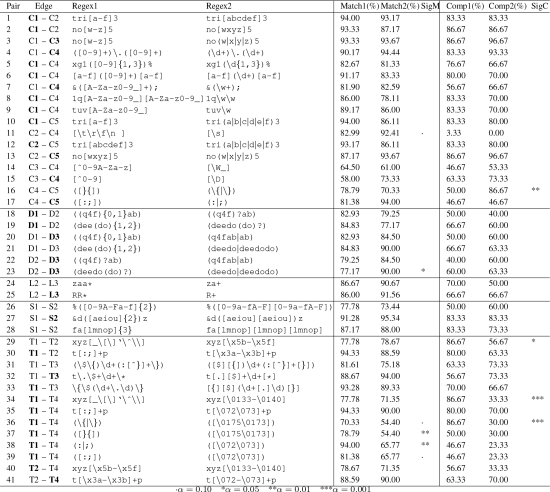
\includegraphics[width=1\textwidth]{table3.png}
	\caption{Párové porovnávanie regexov. Každá hodnota porovnania alebo zloženia je vypočítaná na základe približne 30 dátových bodov od 30 účastníkov štúdie \cite{Chapman2017}}
	\label{fig:table3}
  \end{figure}
\\
V prípade párov 16, 29, 34 a 36 je rozdiel v zložení významný pri $\alpha$\textless0,05, čo naznačuje rozdiely v prospech C5 oproti C4, T1 oproti T2 a dvakrát v prospech T1 oproti T4. V prípade dvojíc 23, 37 a 38 je rozdiel v zhode významný pri $\alpha$\textless0,05, čo naznačuje rozdiely uprednostňujúce D3 pred D2 a dvakrát uprednostňujúce T1 pred T4. Zaujímavé je, že v prípade dvojíc 16 a 29 sú síce rozdiely v zložení významné, ale medzi metrikami zloženia je rozpor. Je potrebné ďalšie skúmanie, aby sme pochopili, za akých okolností sú metriky vo vzájomnom konflikte. Pripomeňme si, že účastníci mohli vybrať neistotu, či sa reťazec zhoduje so vzorom. Z hľadiska porozumenia to naznačuje určitú úroveň zmätku. Pre každý vzor sme spočítali počet odpovedí, ktoré obsahovali aspoň jednu neistotu. Celkovo najvyšší počet neistých odpovedí pochádzal zo vzorov T4 a T2, ktoré majú osmičkovú a šesťuholníkovú reprezentáciu znakov. Najmenší počet neistých odpovedí bol v L3 a D3. Tieto výsledky odrážajú analýzu zrozumiteľnosti, keďže T4 a T2 majú vo všeobecnosti nižšiu mieru zrozumiteľnosti a L3 a D3 vo všeobecnosti vyššiu.\cite{Chapman2017}\\\\

Hoci ANOVA naznačuje, že rozdiely v párovaní sú spôsobené všetkými tromi faktormi, reprezentáciou, veľkosťou DFA a dĺžkou regexu, nie je úplne jasné prečo. Rozptyl v zložení ovplyvňuje len veľkosť DFA. Medzi veľkosťou DFA a zložením existuje silná, pozitívna korelácia pri $\alpha$=0,01 s $\rho$=0,354. Na prvý pohľad sa tento výsledok môže zdať kontraintuitívny, ale vzhľadom na to, že väčšie DFA môžu predstavovať obmedzenejšie regexové jazyky (t. j. jazyky, ktoré akceptujú menej reťazcov), môže byť pre ne jednoduchšie skladať reťazec. Keďže však skúmaný rozsah veľkosti DFA bol od dvoch do ôsmich uzlov, tieto výsledky sa nemusia zovšeobecniť na väčšie regexy. Žiadna z ostatných korelácií nie je významná s $\alpha$\textless0,05.\cite{Chapman2017}

\subsection{Zhrnutie}
Na porovnávanie a skladanie má vplyv veľkosť DFA a na porovnávanie má vplyv aj dĺžka regexu a jeho reprezentácia, čo potvrdzuje, že reprezentácia regexu má vplyv na porozumenie. Čím väčší bol DFA, tým ľahšie bolo pre komunitu generovať reťazce, ktoré mu zodpovedajú. Zdá sa tiež, že existuje jasný trend uprednostňovania T1 pred T4. Uprednostňované sú aj reprezentácie D3 a C5. Hoci sa uprednostňuje porovnanie C1 oproti C2, C4 a C5, žiadne z nich nie je významné.\cite{Chapman2017}

\section{Záver} \label{zaver} % prípadne iný variant názvu
Záver.

%\acknowledgement{Ak niekomu chcete poďakovať\ldots}


% týmto sa generuje zoznam literatúry z obsahu súboru literatura.bib podľa toho, na čo sa v článku odkazujete
\bibliography{literatura}
\bibliographystyle{plain} % prípadne alpha, abbrv alebo hociktorý iný
\end{document}